%\documentclass[12pt]{apa7}
\documentclass[man, noextraspace, floatsintext, 12pt]{apa7}
%\documentclass[12pt, noextraspace, floatsintext]{apa6}
%\documentclass[man, 12pt, noextraspace, floatsintext]{apa6}
%\documentclass[11pt]{article}

% ADD REVIEWING PACKAGE
\usepackage{easyReview}
% Show reviews/edits or not?
\setreviewson
%\setreviewsoff
% Line numbers for ease of pointing to lines
\usepackage{lineno} %[pagewise]
%\linenumbers

\usepackage{lscape}
%Math typesetting packages
\usepackage{amsfonts, amssymb, amsmath, latexsym, amsthm}
%for URLs in-text 
\usepackage{url}
% ================
% = Bibliography =
% ================
%APA style citations and references
%\usepackage[utf8]{inputenc}
%\usepackage{babel,csquotes,xpatch}
\usepackage[backend=biber, style=apa, natbib, sortcites]{biblatex}
\addbibresource{references.bib}

%\usepackage[natbibapa]{apacite} 
% for hanging-indentation style using apacite
%\setlength{\bibindent}{2.5em}
%\setlength{\bibleftmargin}{0em}
% ==========
% = Floats =
% ==========
\usepackage{float}
% include external pictures
\usepackage{graphicx} %Graphics/figures
% rotate figures/tables
\usepackage{rotating} 
% For professional tables
\usepackage{booktabs,threeparttable, multirow} 
\usepackage{tabularx}
% For fixing the column widths
\usepackage{array}
\newcolumntype{L}[1]{>{\raggedright\let\newline\\\arraybackslash\hspace{0pt}}m{#1}}
\newcolumntype{C}[1]{>{\centering\let\newline\\\arraybackslash\hspace{0pt}}m{#1}}
\newcolumntype{R}[1]{>{\raggedleft\let\newline\\\arraybackslash\hspace{0pt}}m{#1}}

% ===================
% ==== Tikz Diagrams	==
% ===================
\usepackage{tikz}
\usetikzlibrary{calc,arrows,positioning,shapes,shapes.gates.logic.US,trees, intersections}
% =======================
% === Other useful packages ==
% =======================
\usepackage[T1]{fontenc} 
\usepackage{placeins}
\usepackage{hyperref}
% subcaptions/subfigures %,justification=centered
\usepackage[hypcap=true,width=\textwidth]{subcaption}
% =============
%  == formatting ==
% =============
% \usepackage[margin=1in]{geometry}
% \setlength{\parindent}{0.5in}
\usepackage{setspace}
% \doublespacing

% ==========
% = Syntax =
% ==========
% For Computer Code in Appendix. I set the language for R, so will need to be changed for different languages
\usepackage{listings}
\lstset{
    language=R,
    basicstyle=\small \ttfamily,
    commentstyle=\ttfamily ,
    showspaces=false,
    showstringspaces=false,
    showtabs=false,
    frame=none,
    tabsize=2,
    captionpos=b,
    breaklines=true,
    breakatwhitespace=false,
    title=\lstname,
    aboveskip=10pt,
    belowskip=-10pt,
    %escapeinside={},
    %keywordstyle={},
    %morekeywords={}
    }%
%~~
\title{Assessing local fit by approximating probabilities}
\shorttitle{Assessing local fit} % For APA package
\author{R. Noah Padgett}
%\author{Graduate Student}
\authorsaffiliations{Baylor University}
%\affiliation{REMOVED FOR PEER REVIEW}



\abstract{Validity evidence for factor structures underlying a set of items can come from how well a proposed model reconstructs, or fits, the observed relationships.
Global model fit is limited in that some components of the proposed model fit better than other components.
This limitation has lead to the recommendation of examining fit locally within model components.
We describe a new probabilistic approach to assessing local fit using a Bayesian approximation, and illustrate use with a simulated dataset.
We show how the posterior approximation closely approximated the sampling distribution of the true parameter.
We discuss potential limitation and possible generalizations.
%\singlespacing
 } % End abstract

\keywords{local fit, factor analysis, Laplace, posterior probability}

%\authornote{REMOVED FOR PEER REVIEW}
\authornote{
R. Noah Padgett, Department of Educational Psychology, Baylor University.

Correspondence concerning this article should be address to R. Noah Padgett, Department of Educational Psychology, One Bear Place \# 97304, Baylor University, Waco, TX 76798. Contact: \href{mailto:noah\_padgett1@baylor.edu}{\tt noah\_padgett1@baylor.edu}
}


\begin{document}

\maketitle

%% Spacing for Eqations Can't be in preamble...
\setlength{\abovedisplayskip}{3pt}
\setlength{\belowdisplayskip}{3pt}

Most methodologists would likely agree that statistical models are an approximation of the process that generated the data we observed.
Structural equation models are no exception to this point.
The approximation of reality has been described as arising from distributional and structural approximations \citep{Bollen2019}.
Identifying these model misspecifications can be at best difficult and at worst impossible.
The task of trying to find evidence for a proposed model is then our focus, and a variety of methods have been developed to help this decision making process.

One popular method of finding evidence for once's proposed model is the use of global fit indices.
Global fit indices help identify whether the model specified as a whole \textit{well} approximates the data generating process.
Typically used indices are the comparative fit index \citep{Bentler1990}, RMSEA \citep{Browne1992}, and SRMR \citep{Bentler1995, Maydeu2018, Joreskog1981}.
Many of these indices are now automatically computed in most SEM software.
However, these indices only provide a coarse estimate of model-data fit \citep{Steiger2007}.

One difficulty comes when the global fit indices are below acceptable (whatever this means to the researcher) and then trying to remedy the misspecification is a systematic and defensible manner.
The global fit indices don't necessarily help us identify where the misspecification is occurring, though.
Presumably, some parts of the model are better representing the latent structure than other parts, but identifying which parts are not representative is not straightforward.
Methods of identifying the source of misfit include investigating residual matrices \citep{Kline2015, Maydeu2017}, modification indicies \citep{Sorbom1989, Kaplan1989}, Wald tests \citep{Wald1943, Buse1982}, likelihood ratio tests \citep{Neyman1928, Buse1982}, and model-implied instrumental variables \citep{Bollen1995, Bollen2019}.
Each method has benefits and pitfalls that need to be considered when looking for evidence of model-data fit. 
The methods above generally provide users with a way of either identifying which specific relationships among observed that are not capture by the model (e.g., residuals) or which specific component of the model that doesn't fit well (e.g., Wald tests).
Once a change in the model has been conducted, a researcher can then compare the results of local fit to see if fit improved.

Evaluating the change in model fit has been helpful for many in the model fit evaluation process. 
But, this process is not without potential drawbacks.
For example, modification indices can lead to conflicting information about sources of misfit leading to statistically equivalent models.
Adding too many paths can lead to over fitting to the observed data and difficulty in interpretation.
Aside from investigating standardized residuals \citep{Maydeu2017}, most current methods of investigating local fit rely on non-intuitive metrics (e.g., modification indices, likelihood ratios, or p-values); however, we are proposing a more directly interpretable approach using probabilities for local fit assessment. 
We aim to develop a probabilistic approach to approximate whether additional paths will result in meaningfully interpretable contribution to the model.
With our method, we aim to help control against over fit and aid interpretation driven local fit assessment.

The main contributions of this research are: First, we extend previous research on local fit assessment by introducing a probabilistic method and the describe the conditions in which this approach holds theoretically reliable results. 
Second, we demonstrate the application of this approach in a simulated dataset with a known latent structure.
Finally, we investigated the performance through Monte Carlo simulation study evaluating the accuracy of the predicted probabilities.

\subsection{Proposed Probabilistic Method}

Local fit assessment by means of investigating residual matrices, modification indicies, Wald tests, likelihood ratio tests or model-implied instrumental variables has been shown to provide useful information in a variety of contexts \citep{Chou1990, Whittaker2012, Maydeu2017}.
However, we were still left in a bit of quandary as to whether any potential changes would be of a substantive importance.
We have developed a hopefully straightforward approach to tackling this aspect of local fit evaluation by means of in iterative approximation of the non-estimated parameters.
In our experience, we have found that the model changes proposed through modification indices results in parameter estimates that were of little substantive meaning.
For example, a cross-loading that is low or a residual covariance that suggests a weak relationship that substantively doesn't add to our understanding of the measurement of the construct of interest.

We propose a method that approximates what the magnitude of the non-estimated parameters would be and to couch the estimates in terms of the probability that the parameter is of substantive interest.
The idea is to define a region of the parameter space that we would consider to be of substantive meaningfulness.
A natural choice in the case of factor loadings is to define the region as $\vert \lambda \vert \geq 0.32$, which is the threshold typically considered as the bound for standardized factor loadings in exploratory factor analysis.
However, we are not restricted to this region; for example, we might be interested in knowing if any loadings would likely be greater than $1$, indicating that the item loads more strongly than the item we fixed for identification.
This approach of approximating regions is similar to defining a ``region of practical equivalence (ROPE)'' described in \textcite{Shi2019} as a Bayesian approach for measurement invariance testing.
The ROPE is a region in the parameter space that the researcher determines to be insignificant, and this is already done in most applications of exploratory factor analysis (EFA) when the researcher suppresses factor loadings that are below 0.32 \citep{Benson1998}.

Our idea boils down to defining regions of the parameter space that are of practical insignificant and then approximate the probability that our model parameters fall in that space.
The approximation we are proposing is based on a rough approximation of a posterior distribution to compute probabilities based on Bayes theorem.
A similar quantity often of interest in Bayesian methods is the posterior predictive probability \citep[PPP or $p$-value, ][]{Gelman1996, Rubin1996}.
The PPP is often used to construct probabilistic inferences about test statistics from the posterior predictive distribution.
However, for the current application we are interested in computing a probability based on the posterior itself leading to a simpler approximation problem.
The proposed local fit assessment builds on this idea of approximating the posterior probability associated the parameters.
 
A similar approach of assessing model fit was discussed by \textcite{Lee2016}.
The authors used a similar posterior approximation to help evaluate global model fit and identify influential observations.
The authors hinted that the probabilistic approach can be used to assess model fit in a variety of ways such as residual covariances.
However, to date no one has built on this method for investigations of local fit assessment and is the focus of our work.
Next, we introduce the Bayesian ideas needed to build up the approach. 

\subsubsection{Introduction to Bayesian Approach}

Bayes theorem is one of the most powerful tools to manipulate probabilities. 
Bayes theorem lets us decompose a conditional probability into a likelihood statement about our data and a hypothesized probability space for model parameters (i.e., the prior). Or, more formally as
\begin{align*}
p(\theta \vert Y) \propto \ell (Y \vert \theta)p(\theta)
\end{align*}
where $\propto$ is read as ``proportional to'', $\ell (Y \vert \theta)$ is the likelihood of the data $Y$ determined by the model specified and parameters $\theta$, and $p(\theta)$ is the joint prior distribution for the parameters in the model.
The posterior is usually sampled from using Monte Carlo methods (e.g., Gibbs sampling, Hamiltonian Monte Carlo, etc.).
However, in this case we elect to utilize a \textit{relatively} simple approximation of the posterior that we can sample from relatively quickly.

Under mild regularity conditions the posterior distribution for $\theta$ will approximate a normal distribution as the number of samples drawn from the distribution increases \citep{DBA3}.
Using this property of the posterior, we can use Laplace's method to derive a second-order Taylor series approximation to the posterior \citep{Tierney1986}.
The Taylor series approximation is used to get a point estimate for the posterior expectation and variance.
Then, using these two pieces matched with the knowledge that the posterior is asymptotically normally distributed, we arrive at an approximate posterior distribution for any parameter. 
The approximation is known to provide a useful approximation of posteriors for relatively simple models in a variety of contexts \citep{Kass1989, Rue2009}.

Under the same regularity conditions that allow us to assume the normal distribution we would get that that $\hat{\theta}$ under the Laplace approximation is nearly equal to $\hat{\theta}_{MLE}$ and that the variance under the Laplace approximation is nearly identical to the $I_{OBS}$  (the observed information). %$\hat{\theta} \approx \hat{\theta}_{MLE}$ and that $-\ddot{q}(\hat{\theta}) \approx I_{OBS}$ (the observed information).
Not including the prior distribution for $\theta$ has been done previously \citep{Lee2016, Rue2009, Wolfinger1993, Li1992}.
This would decrease our uncertainty in the posterior distribution for $\theta$ even if only slightly.
Additionally, utilizing a minimally informative prior structure provides a useful initializing point for numerical methods.
Next, we will describe how we can utilize Laplace's method in factor analysis for local fit assessment.

\subsubsection{Applying Laplace Approximation to CFA}

We borrowed most notation for Bayesian factor analysis from the chapter ().
 We can take the traditional factor model (shown below) and restructure the model to be able to efficiently approximate posterior features of interest.
Full model is
\begin{align*}
\mathbf{Y}_i &= \tau + \Lambda \eta_i + \theta_i\\
\Sigma &= \Lambda^T \Phi \Lambda + \Theta\\
\mathbf{Y}_i &\mid \tau, \Lambda, \eta_i, \Theta \sim \mathrm{N}\left(\tau + \Lambda \eta_i, \Theta \right)\\
\eta_i &\mid \kappa, \Phi \sim \mathrm{N}\left(\kappa, \Phi \right)
\end{align*}
where $\mathbf{Y}_i$ is the response vector for person $i$, $\tau$ is the vector of indicator intercepts, $\Lambda$ is the matrix of factor loadings, $\eta_i$ is the vector of factor scores, $\theta_i$ is the vector of residuals, $\Sigma$ is the indicator/observed variable covariance matrix, $\Theta$ is the error covariance matrix, $\kappa$ is the vector of factor intercepts (usually fixed to 0), and $\Phi$ is the factor covariance matrix.
Which is a pretty large model with a lot of potential parameters and moving pieces.
The full model could be incorporated in a Bayesian perspective relatively easily, but the parameter space grows rapidly.
Below is one potential way the full joint posterior could be express.
\begin{align*}
\pi\left(\tau, \Lambda, \eta,\Theta, \kappa, \Phi\mid \mathrm{Y}\right) \propto \ell\left(\mathrm{Y} \mid \tau, \Lambda, \eta,\Theta, \kappa, \Phi\right) \times \pi\left(\tau, \Lambda, \eta,\Theta, \kappa, \Phi\right)
\end{align*}
Which is pretty gnarly if there are a large number of subjects, items, and latent variables.
The likelihood is not difficult to define due to the assumption of conditional independence of subjects, and even further simplification can be made if conditional independence of items is assumed (i.e., $\Theta$ is a diagonal matrix)
\begin{align*}
\ell\left(\mathrm{Y} \mid \tau, \Lambda, \eta,\Theta, \kappa, \Phi\right) &= \prod_{i=1}^{N} f\left(\mathbf{Y}_i \mid \tau, \Lambda, \eta_i, \Theta \right)\\
 &=\prod_{i=1}^{N} \prod_{j=1}^{J}f\left(Y_{ij} \mid \tau_j, \lambda_{j}, \eta_i, \theta_{jj} \right)
\end{align*}
which results in a nice linerization of the complex looking likelihood that we started with.
But, the more complicated issue is on the construction of the joint prior distribution.
Constructing joint prior distributions directly is typically not possible outside of special cases (e.g, normal-gamma conjugate prior in normal theory multiple linear regression) in multiparameter problems.

In multiparameter problems, a common method for building the join prior distribution is to construct the prior hierarchically.
The hierarchical prior for factor models can be constructed by decomposing the prior into parameter groups that can defensibly be independent or at least conditionally independent.
A potential decomposition is to have independent groups for factor loadings ($\Lambda$), item intercepts ($\tau$), and error (co)variances ($\Theta$), then group the factor scores ($\eta$), factor intercepts ($\kappa$), and factor covariance matrix ($\Phi$) together.
The later grouping can be structured where the factor scores distribution is conditional on the factor intercept and factor covariance matrix priors.
The decomposed prior could look something like this
\begin{align*}
\pi\left(\tau, \Lambda, \eta,\Theta, \kappa, \Phi\right) &= \pi\left(\eta, \kappa, \Phi\right)\pi\left(\tau\right)\pi\left(\Lambda\right) \pi\left(\Theta\right)\\
&= \pi\left(\eta\mid \kappa, \Phi\right) \pi\left(\kappa\right)  \pi\left(\Phi\right) \pi\left(\tau\right)\pi\left(\Lambda\right) \pi\left(\Theta\right).
\end{align*}
Some common specifications of the priors for these parameters are
\begin{align*}
\eta\mid \kappa, \Phi &\sim \mathrm{N}(\kappa,\Phi)\\
\kappa &\sim \mathrm{N}(\mu_{\kappa}, \sigma^2_{\kappa})\\
\Phi &\sim \mathrm{Inverse-Wishart}(d\Phi_0, d),\ d \geq M\\
\tau{j} &\sim \mathrm{N}(\mu_{\tau}, \sigma^2_{\tau})\\
\lambda_{jm} &\sim \mathrm{N}(\mu_{\lambda}, \sigma^2_{\lambda})\\
\theta_{jj} &\sim \mathrm{Inverse-Gamma}(\alpha_{\theta}, \beta_{\theta}).
\end{align*}
The indices $j$ correspond to the $j^{th}$ indicator and $m$ is index over latent variables.
The factor loadings, intercepts, error (co)variances may be specified independently for each individual parameter which greatly simplifies the process, but is not necessary.
If one had a belief that the error (co)variance matrix was not diagonal, then that structure could be included as part of a joint prior on $\Theta$.

Once the joint prior is constructed, one difficult hurdle of a full Bayesian analysis would be to try to sample from the posterior.
This is generally where we would move to some type of Markov Chain Monte Carlo set-up to try to efficiently sample from the marginal posteriors of these parameters.
Some software options that make this job easier include M\textit{plus} \citep{Mplus}, blavaan \citep{blavaan}, JAGS \citep{jags}, OpenBUGS \citep{bugs}, Stan \citep{Stan}, and many more.
However, in this study, we are proposing a drastic simplification of this process to aim a a rough approximation of specific features of the posterior.

As we have described in the section ``Proposed Probabilistic Method'', our aim is to approximate the probability that a parameter is outside a region of practical importance (or that the absolute value exceeds a threshold).
The powerful machinery that is MCMC can certainly be used for this purpose.
However, our intent is to provide a simpler, quicker, and less computationally intensive approach that can be utilized as part of the model evaluation process for local fit assessment.
The complex posterior distribution built up till now is simplified as we shift from sampling from the marginal posterior to a specific conditional posterior for each parameter.
Meaning we sample from each posterior by fixing estimates of loadings, error (co)variances, factor (co)variances, etc. in order to reduce the model down to a single parameter problem.
Then a very simple and generalize-able method is available for approximately sampling from the conditional posterior of parameter(s) of interest.

This approach may work as follows for approximating the posterior of a specific factor loading $\lambda_{z1}$, the $z^{th}$ loading of factor 1.
If we utilize the nice simplifications likelihood that result from the independence assumptions, then the posterior simplifies to the following by conditioning on the fixed parameters that can come from the MLE solution.
\begin{align*}
\pi(\lambda_{z1} \mid \mathbf{\theta}) &= \pi(\lambda_{z1} \mid \tau, \Lambda_{zm \neq z1}, \eta,\Theta, \kappa, \Phi, \mathrm{Y})\\ 
&\propto \ell\left(\mathrm{Y} \mid \tau, \Lambda, \eta,\Theta, \kappa, \Phi\right) \times \pi(\lambda_{z1})\\
&= \prod_{i=1}^{N} f\left(\mathbf{Y}_i \mid \tau, \Lambda, \eta_i, \Theta \right)\times \pi(\lambda_{z1} \mid \mu_{\lambda}, \sigma^2_{\lambda})\\
&= \prod_{i=1}^{N} \prod_{j=1}^{J} f\left(Y_{ij} \mid \tau_j, \lambda_{j}, \eta_{i}, \theta_{jj} \right)\times \pi(\lambda_{z1} \mid \mu_{\lambda}, \sigma^2_{\lambda})\\
&\propto \prod_{i=1}^{N} f\left(Y_{iz} \mid \tau_z, \lambda_{z1}, \eta_{i1}, \theta_{zz} \right)\times \pi(\lambda_{z1} \mid \mu_{\lambda}, \sigma^2_{\lambda})\\
&= \prod_{i=1}^{N} \frac{1}{\sqrt{2\pi \sigma^2_{zz}}} \exp\left\lbrace\frac{-1}{2\sigma_{zz}} \left(Y_{iz} - (\tau_z +\lambda_{z1}\eta_{i1})\right)^2 \right\rbrace \frac{1}{\sqrt{2\pi \sigma^2_{\lambda}}} \exp\left\lbrace\frac{-1}{2\sigma_{\lambda}} \left(\lambda_{z1} - \mu_{\lambda}\right)^2 \right\rbrace\\
&\propto \exp\left\lbrace \frac{-(\sigma_{zz} + \sigma_\lambda \sum \eta_{i1}^2)}{2\sigma_{\lambda}\sigma_{zz}} \left(\lambda_{z1} - \frac{\sigma_{\lambda}\sum y_{iz}\eta_{i1} -\sigma_{\lambda}\tau_{z}\sum\eta_{i1}+\sigma_{zz}\mu_{\lambda} }{\sigma_{zz} + \sigma_\lambda \sum \eta_{i1}^2}\right)^2 \right\rbrace\\
& \therefore\\
\lambda_{z1} &\sim \mathrm{N}(M, V)\\
M &= \frac{\sigma_{\lambda}\sum y_{iz}\eta_{i1} -\sigma_{\lambda}\tau_{z}\sum\eta_{i1}+\sigma_{zz}\mu_{\lambda} }{\sigma_{zz} + \sigma_\lambda \sum \eta_{i1}^2}\\
V &= \left(\frac{\sigma_{\lambda}\sigma_{zz}}{\sigma_{zz} + \sigma_\lambda \sum \eta_{i1}^2}\right)^2
\end{align*} 
which can be reduced more depending on the of priors for the $\lambda_{z1}$.  But, this is not the most helpful given that the posterior depends on the unknown values of the latent variable $\eta$, but thankfully in application we can side-step the need for these values.
Essentially, what we have done above is just a straightforward application of Bayes theorem to get a closed form solution for the posterior.
This is not as simple for the residual covariances, though.
We think the above was mostly just a sanity check to make sure we knew what the math was doing and to show that under the simplifications we're proposing we can arrive at ``nice'' solutions.
But, this is certainly not going to be done in practice given that the posteriors for cross-loadings and (co)variances are typically more difficult to derive depending on the choice of prior.


%~~\\
%Discuss issue of fixing so many parameters, may not be an issue since it is a ``conditional'' posterior, we are simply conditioning on fixed values.
%My method of accounting for the uncertainty in the fixed parameters is the scale the posterior covariance matrix (i.e., the hessian) up by a factor of the number of fixed parameters.
%
%~~\\
%Ideas:\\
%- maybe supply a general algorithm block to describe the code
%
%- The code was written in R \citep{R2020} so that the code can easily build on the lavaan package \citep{lavaan2012}.
%
%- condense code?



\section{Illustrative Example}

So, now to illustrate the method, suppose we have the ``true'' factor model shown in Figure \ref{fig:model}.
A sample of 300 was drawn from this population.
We simplified the model here for illustration of our approach to local fit assessment.
\begin{figure}
\centering
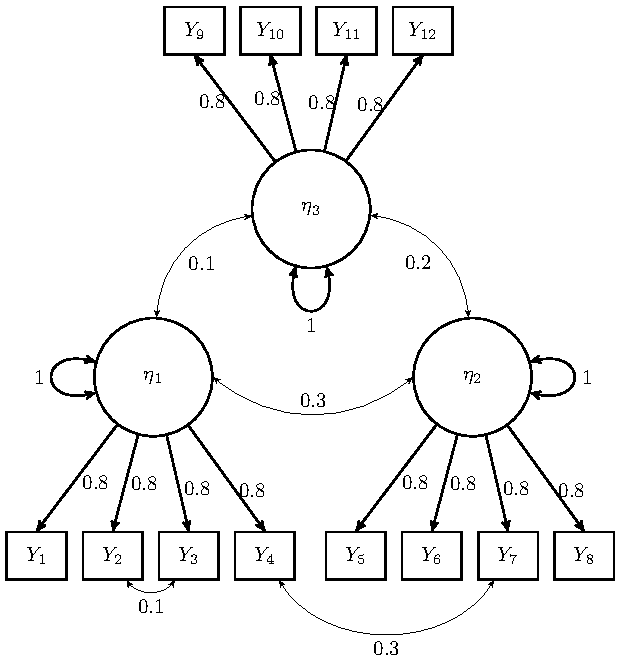
\includegraphics[width=0.5\textwidth]{fig/sim_factor_structure_values}
\caption{Simulating data model}
\label{fig:model}
\end{figure}
Using this sample, a factor analysis without the residual covariances was fit to these data using \textsf{lavaan} \citep{Rosseel2012}.
We found evidence that the model does not fit these data $(\chi^2(51) = 72.8, p = 0.024)$.
Now the task is to try to find out which relationships we are missing or have underestimated according to our model.
Next, we applied the described probabilistic approach to try to identify likely omitted paths that are the source of misfit.
These results are shown next whether the paths identified as most likely are shown in descending order. 
For simplicity we are only showing the paths that had probabilities greater than 0.10 (i.e., 100 out of 1000 draws from the posterior were outside the region of practical equivalence).
These estimates are shown in Table \ref{tb:prob}.
We found that, with the method described in this paper, the two paths with the highest probability of being meaningful in magnitude are the two residual covariances that were in the population model.


\begin{table}[ht]
\centering
\caption{Estimated probabilities of parameters being outside region of practical equivalence}
\label{tb:prob}
\begin{tabular}{lr}
  \toprule
Parameter ($\theta$) & $\mathrm{Pr}( \mid \theta \mid \geq cutoff)$\\ 
  \midrule
  $\mathrm{cov}(y_7, y_4)$ & 0.810 \\ 
  $\mathrm{cov}(y_3, y_2)$ & 0.461  \\ 
  $\mathrm{cov}(y_{12}, y_7)$ & 0.254 \\ 
  $\mathrm{cov}(y_9, y_4)$ & 0.233 \\ 
  $\mathrm{cov}(y_4, y_2)$ & 0.221 \\ 
  $\mathrm{cov}(y_{10}, y_1)$ & 0.201  \\ 
  $\mathrm{cov}(y_9, y_1)$ & 0.191  \\ 
  $\mathrm{cov}(y_9, y_7)$ & 0.164  \\ 
  $\mathrm{cov}(y_9, y_8)$ & 0.161  \\ 
  $\mathrm{cov}(y_4, y_1)$ & 0.160  \\ 
  $\mathrm{cov}(y_3, y_1)$ & 0.147  \\ 
  $\mathrm{cov}(y_9, y_2)$ & 0.126  \\ 
  $\mathrm{cov}(y_{10}, y_5)$ & 0.108  \\
   \bottomrule
\end{tabular}
\end{table}


\section{Simulation Study}

In this simulation study, we evaluated the estimated probabilities against the sampling distribution of the parameters.
To do so, we generated 10,000 datasets from the population model, fit the population model to each, and extracted the sampling distribution of the model parameters.
We compared the sampling distribution to the approximated empirical sampling distributions used to compute the approximating probabilities shown in Table \ref{tb:prob}.
We focused on the two residual covariances from the model in Figure \ref{fig:model}, because these two parameters are likely to be initially omitted from a model specification.

The true and approximated sampling distributions are shown in Figure \ref{fig:dist}.
The probabilities from the ``true'' sampling distribution are ${\rm Pr}(\mathrm{cov}(y_7, y_4) > 0.25) = .82$ and ${\rm Pr}(\mathrm{cov}(y_3, y_2) > 0.25) = .72$.
We found relatively major difference between the true and approximated sampling distribution for $\mathrm{cov}(y_3, y_2)$ and the probability.
This is in contrast to the nearly perfectly matched distribution for $\mathrm{cov}(y_7, y_4)$.

\begin{figure}
\centering
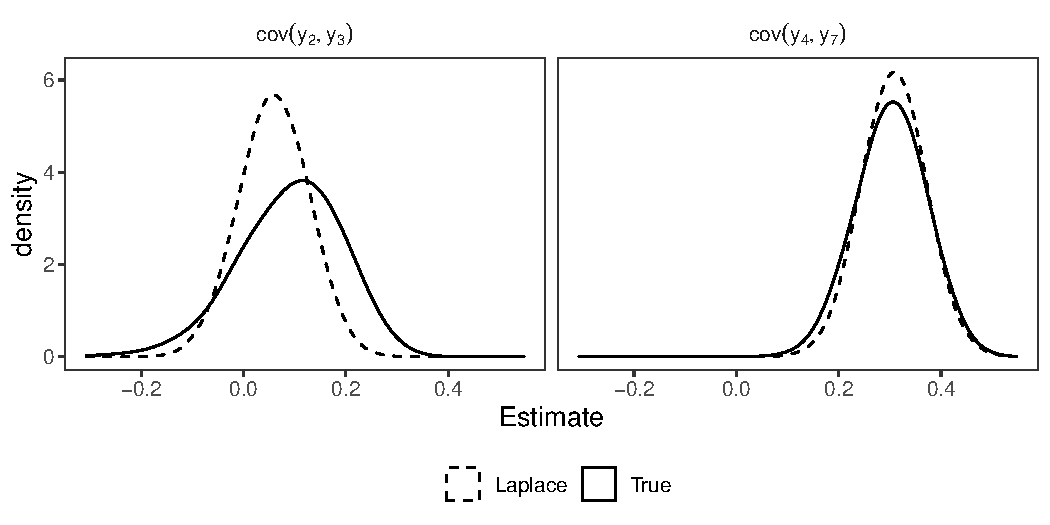
\includegraphics[width=0.9\textwidth]{fig/sampling_dist}
\caption{True and approximated sampling distributions for model residual covariances}
\label{fig:dist}
\end{figure}


\section{Discussion}

In this paper, we have outlined our method investigating local fit by approximating the probability that a parameter is meaningfully different than zero.
We built our approach on similar ideas of model fit by \textcite{Lee2016} and \textcite{Shi2019}.
By utilizing a Bayesian perspective, the resulting probability is intuitive to interpret.
A result that doesn't require a complex interpretation provides a nice compliment to existing methods of model modification \citep[e.g., ][]{Sorbom1989, Kaplan1989, Wald1943}.
We avoided some of the complexities of estimation by using a straightforward approximation based on Laplace's method.
The approximation is also relatively fast compared to full Markov chain Monte Carlo methods.

Despite some potential advantages of the approach we have developed, we are also aware of some potential disadvantages as well.
One of the issues is trying to decide what value of each parameter should be used for computing the probability? For (standardized) factor loadings, we used a value of 0.32 suggest by \textcite{Benson1998} from EFA, but other values may be of interest.
More work needs to be done to figure out how strong correlations need to be in order to be of interest.
However, these values probably need to change depending on the inferences of interest.
Additionally, we have a similar issue of trying to decide how high does the probability need to be in order for us to have confidence that the omitted path is meaningful? 0.5? 0.4? Maybe this value should be a function of the number of parameters tested, similar to a Bonferroni adjustment.
A set number for this probability may be counter productive since we want to view this probability more as reflective of degree of evidence or belief about the magnitude of the parameter.
We view a higher probability is more evidence that the parameter is of interest.
This is sometimes called the \textit{epistemic} or \textit{degree-of-belief} perspective of probability \citep[][, p.XX]{Levy2016, deFinetti1974}.

We have provided an approach to local fit assessment that allows for more information to be gained about the relationships in our data.
Our proposed approach is intuitive and aligns with aims to search for sources of local fit rather than global fit.
Future work could investigate how this approach could be utilized for parameters included in the model not just the omitted paths.

% ============================= 
\newpage
\raggedright
%\bibliographystyle{apacite} 
% You may have to select another style. Remember: LaTeX, BibTeX, LaTeX, LaTex to get the citations to appear
%\raggedright
%\urlstyle{same}
%\bibliography{references}
\printbibliography
%~~
%%~~
%\appendix
%
%\section{R Code}
%
%Create a self-contained function - will contain subfunctions.

\end{document}
